\subsubsection{Addaccu circuit}

\begin{figure}[h!]
\centering
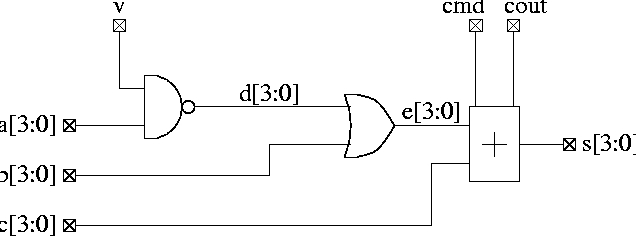
\includegraphics[width=.9\textwidth]{images/add1.png}
\end{figure}
  
\newpage

\subsubsection{Data-path}

\begin{figure}[h!]
\centering
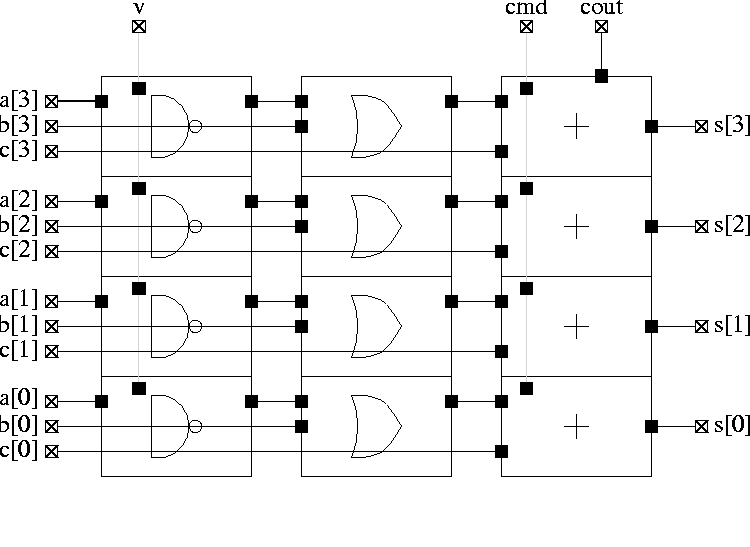
\includegraphics[width=.9\textwidth]{images/add2.png}
\end{figure}

\subsubsection{Description of the circuit with \emph{Stratus}}

\begin{figure}[hbp]
\centering
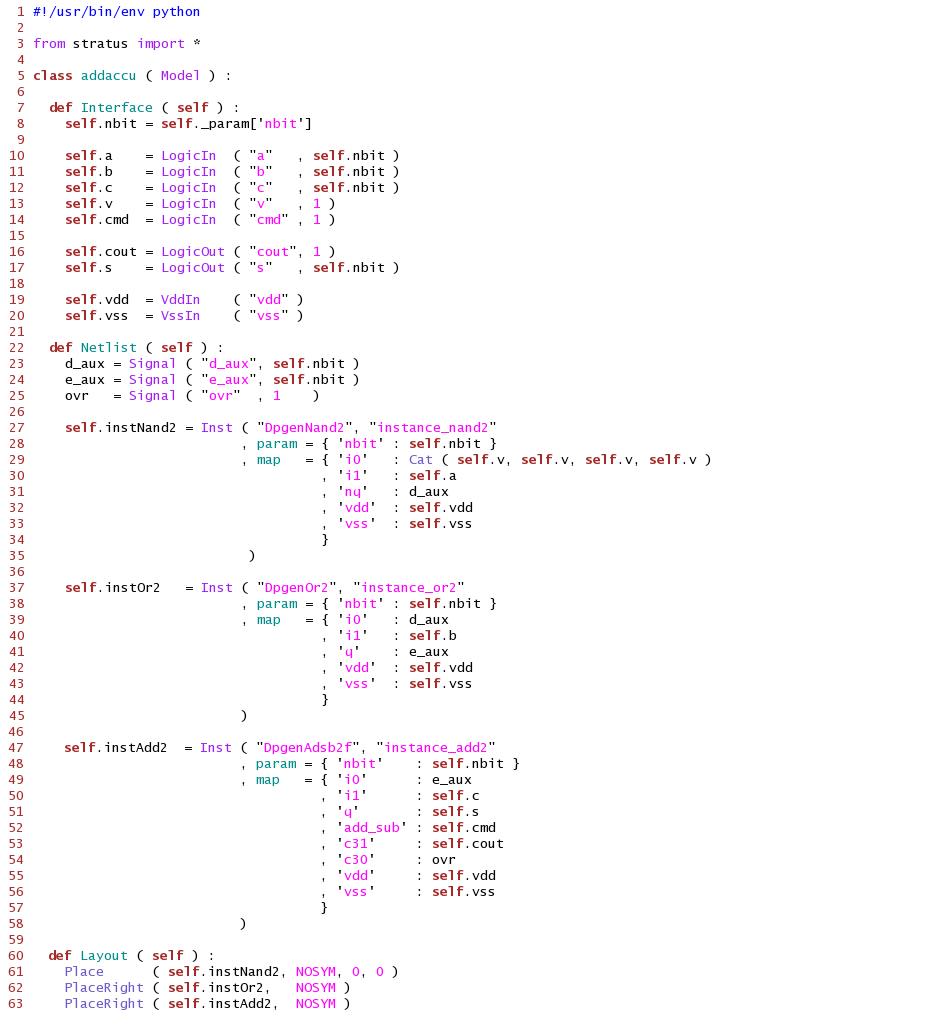
\includegraphics[width=1.2\textwidth]{images/addaccu.png}
\end{figure}

\newpage

\subsubsection{Creation of the circuit}

\begin{figure}[hbp]
\centering
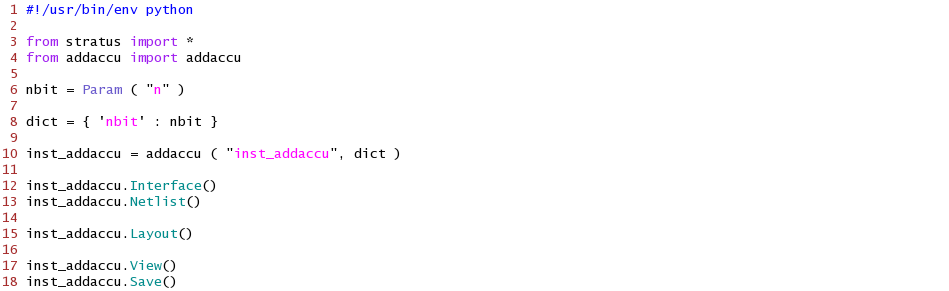
\includegraphics[width=1.3\textwidth]{images/test.png}
\end{figure}

%\newpage
  
\subsubsection{How to execute the file}

\begin{verbatim}
python test.py -n 4
\end{verbatim}
\indent or :
\begin{verbatim}
chmod u+x test.py
./test -n 4
\end{verbatim}

\subsubsection{The editor}

The method \verb-View- permits to open an editor in which one can see the cell being created as shown in the picture below.
\begin{figure}[hbp]
\centering
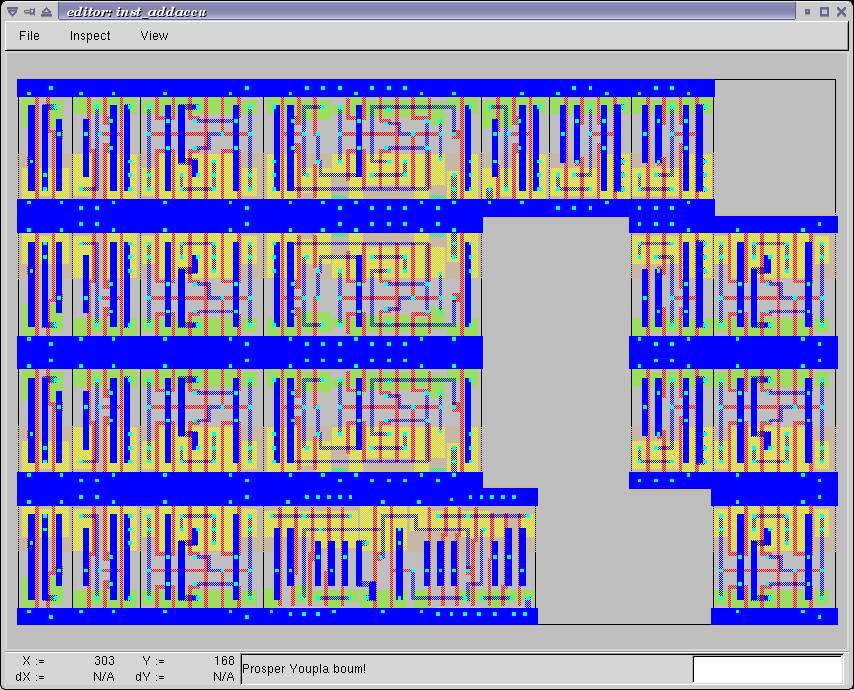
\includegraphics[width=1\textwidth]{images/editor.png}
\end{figure}


\subsubsection{See Also}

\hyperref[ref]{\emph{Stratus}}{}{Stratus}{secstratus}
\hyperref[ref]{\emph{Model}}{}{Model}{secmodel}
\hyperref[ref]{\emph{Param}}{}{Param}{secparam}
\hyperref[ref]{\emph{Netlist}}{}{Netlist}{secnetlist}
\hyperref[ref]{\emph{Layout}}{}{Layout}{seclayout}
\hyperref[ref]{\emph{Place and Route}}{}{Place and Route}{secroute}
\hyperref[ref]{\emph{Facilities}}{}{Facilities}{secfacilities}
